\section{Puzzles}
While exploring the castle, the player can choose to solve some puzzles and, by so, avoid fighting some enemies.

\subsection{Town square}

TODO

\subsection{Castle of Dynamia}

\subsubsection{1. Build a machine}

\begin{figure}[H]
  \centering
  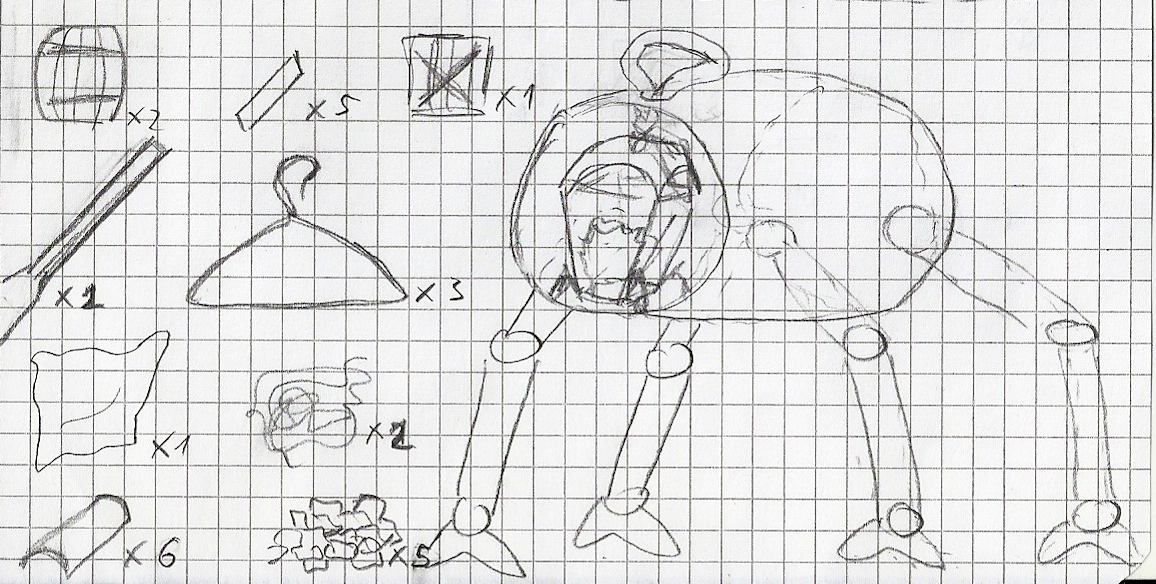
\includegraphics[width=\textwidth]{Images/Puzzles/castleOfDynamia_1}
  \caption{Puzzle 1 in the Castle of Dynamia}
\end{figure}

In order to enter in the courtyard the player can use some debris to build a machine for Calcifer that allows him to climb the wall without being detected.

The player has different parts and he/she has to understand how to combine them. He/She has to break some part to obtain new components. Some parts are not required to build the machine.

\subsubsection{2. Rotate the torch}

\begin{figure}[H]
  \centering
  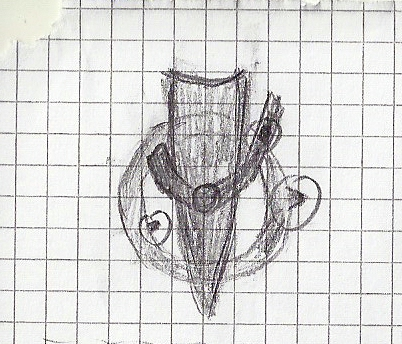
\includegraphics[width=\textwidth]{Images/Puzzles/castleOfDynamia_2}
  \caption{Puzzle 2 in the Castle of Dynamia}
\end{figure}

The torch is a puzzle itself. The player has to rotate the torch and its arms according to the given scheme.

When the player rotates the main body, the two arms rotate too. When he/she rotates an arm, the main body rotates too, but the other arm stays still.

\subsubsection{3. Press the bricks}

\begin{figure}[H]
  \centering
  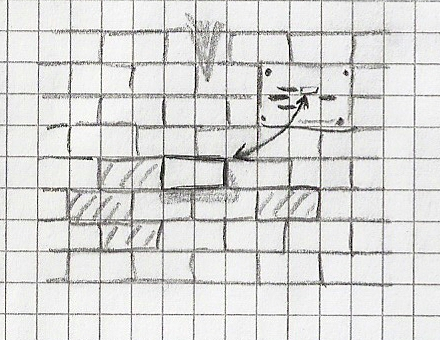
\includegraphics[width=\textwidth]{Images/Puzzles/castleOfDynamia_3}
  \caption{Puzzle 3 in the Castle of Dynamia}
\end{figure}

Near the torch there is a small plate with some horizontal lines. The player has to press the bricks in the corresponding position under the torch.

A protruding brick helps the player to identify the bricks to press.

\subsubsection{4. Connect the cables}

\begin{figure}[H]
  \centering
  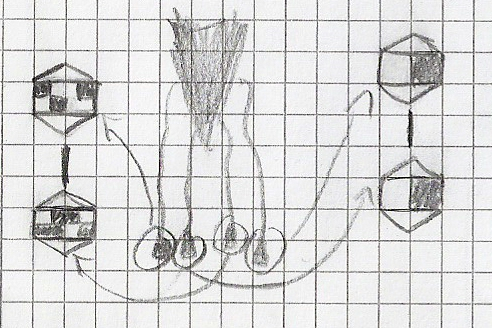
\includegraphics[width=\textwidth]{Images/Puzzles/castleOfDynamia_4}
  \caption{Puzzle 4 in the Castle of Dynamia}
\end{figure}

There are some cables that hang under the torch. The player has to connect them in the correct pairs, according to the pattern on the plugs.

